Liquid Xenon (LXe) is an ideal target for rare event detection, and is particularly well suited for WIMP searches. Xenon is an excellent scintillator, highly transparent to its own scintillation light. It is readily available on the market with a typical world production rate of about 65 tonnes/year. Xenon can be effectively purified for particle detector applications in the multi-tonne range. The high density of LXe allows for the construction of compact detectors that feature a low-background inner core due to the large atomic number of xenon and the absence of significant long-lived radioisotopes. The mean free path of high-energy gamma rays from natural radioactivity in detector materials is typically much smaller than the detector size, so that the former interact in the outermost region of the target (self-shielding), enabling for their efficient removal in offline data analysis. When combined with a technology capable of position reconstruction, namely a two-phase Time Projection Chamber (TPC), this allows the definition of a low-background inner fiducial volume that is used for rare event searches.

\begin{figure}[!htbp]
\begin{center}
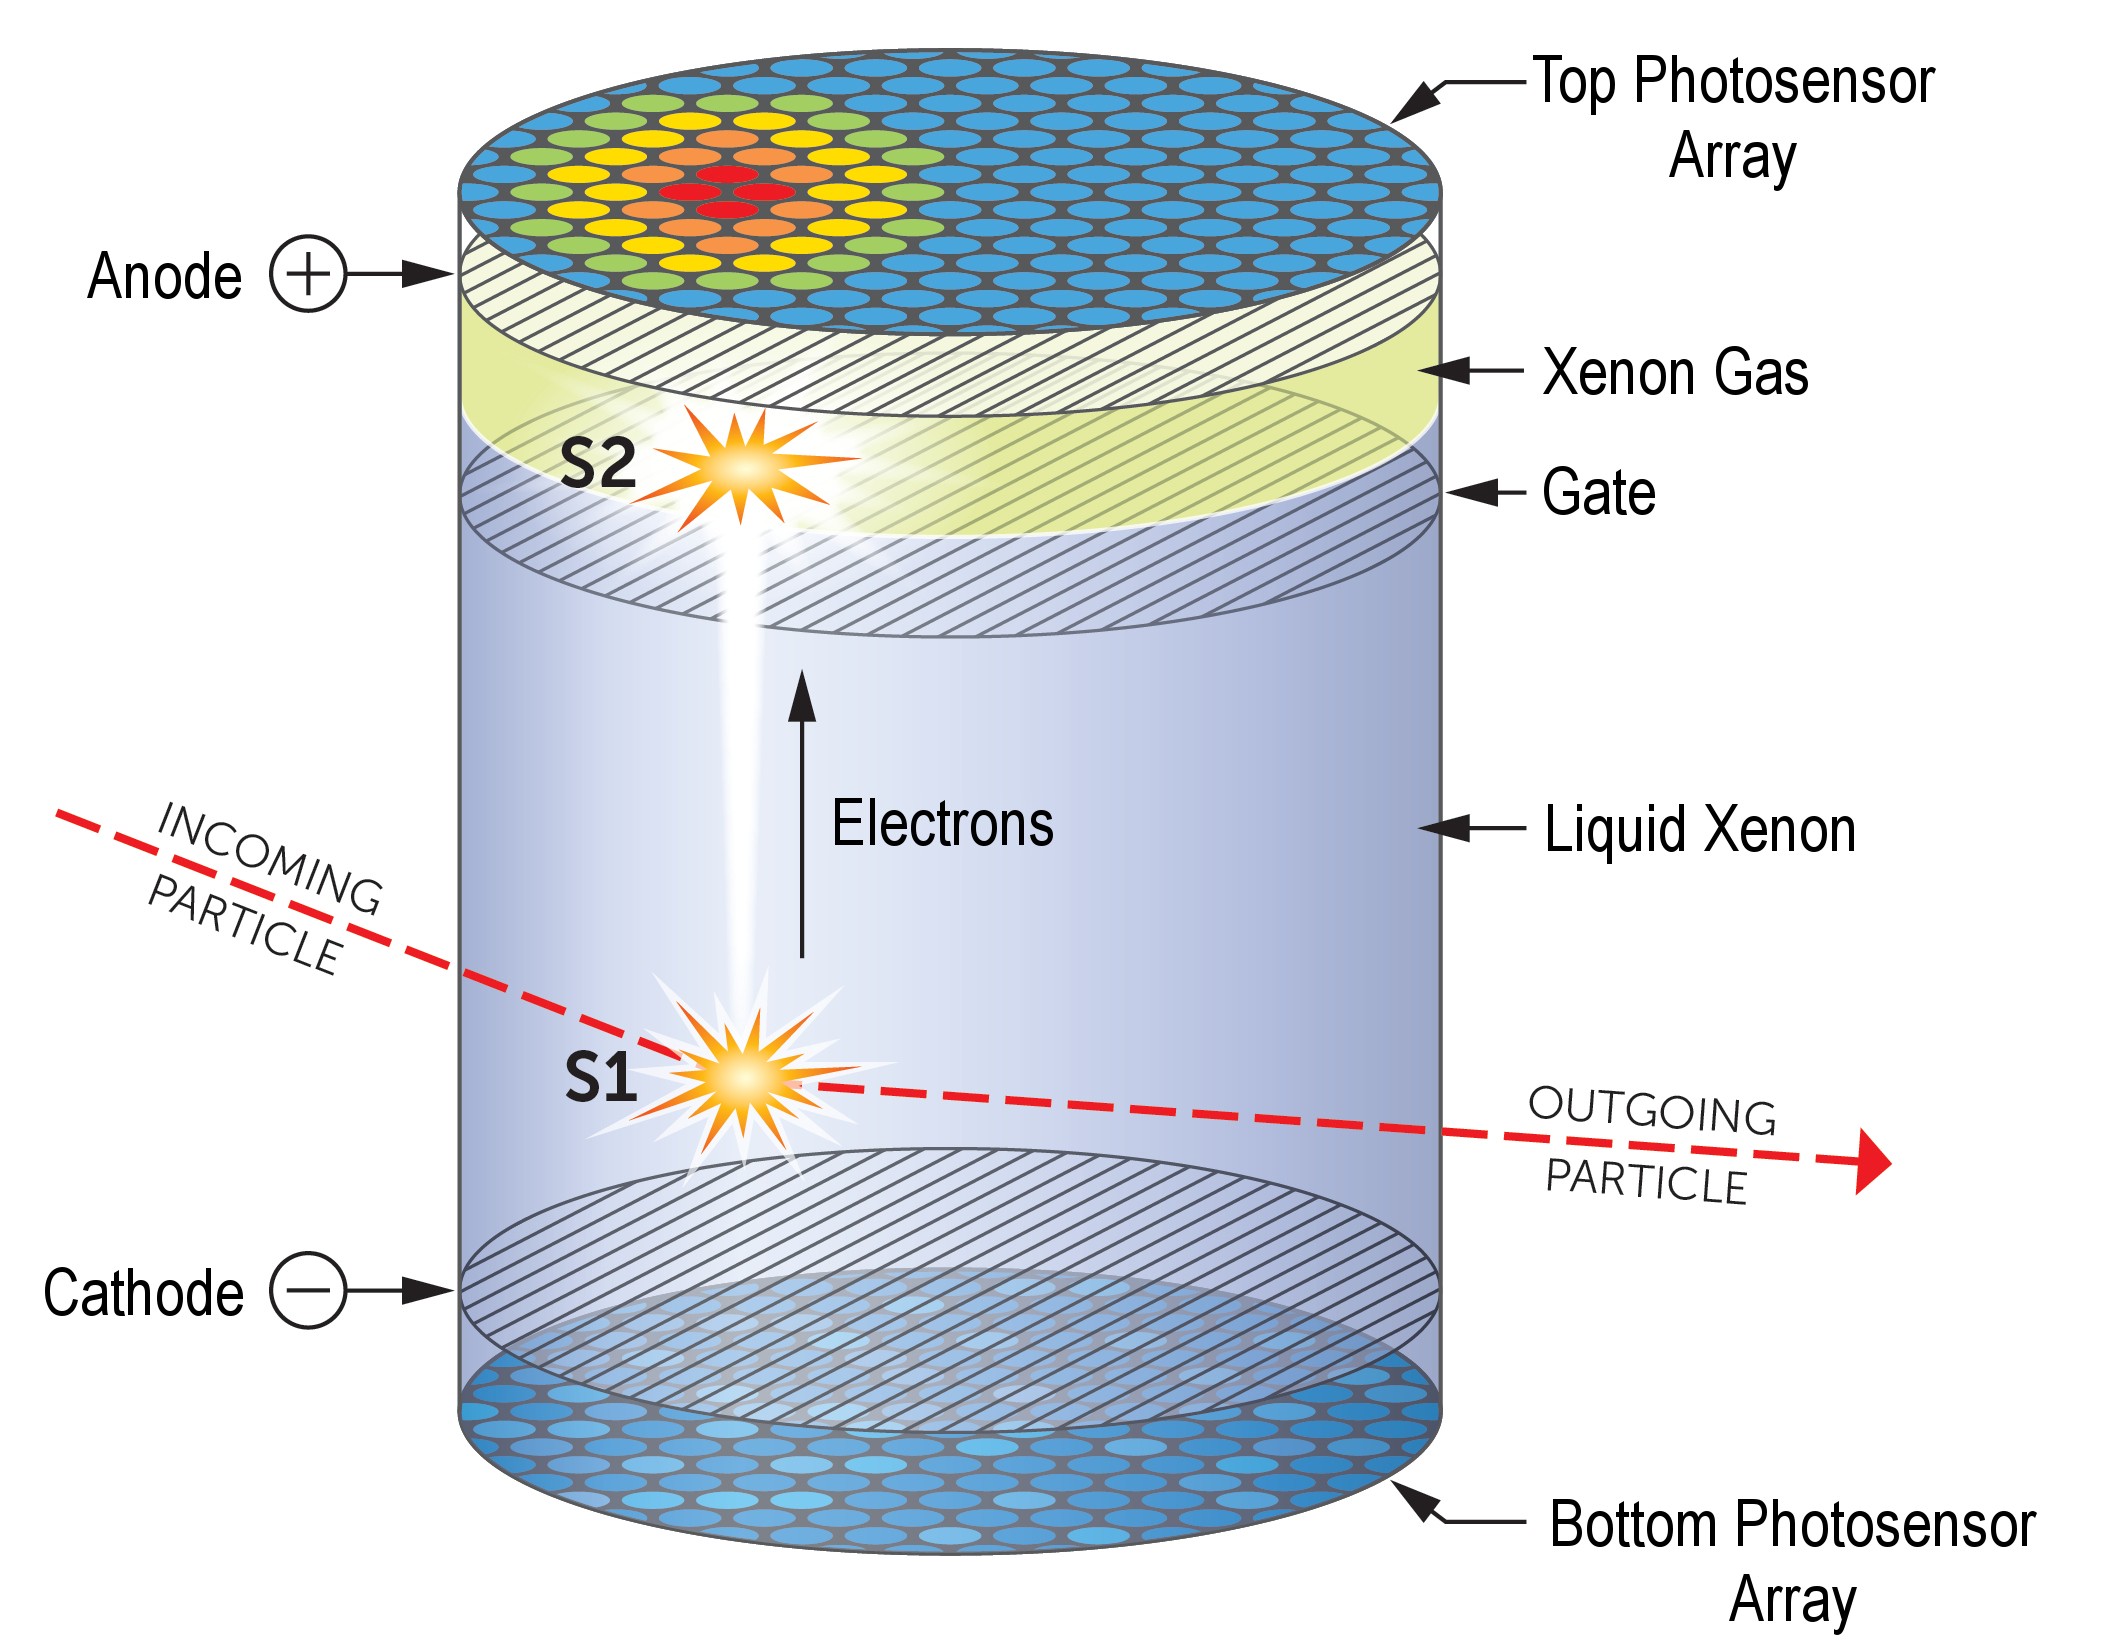
\includegraphics[width=0.99\columnwidth]{figures/xenon_fig_tpc-mo_lifton.jpg}
\caption{Principle of a dual-phase liquid xenon time projection chamber. Energy from a particle interaction within the active liquid xenon volume produces prompt scintillation light (S1) and a delayed  signal (S2) from electroluminescence (proportional scintillation) in the gaseous xenon layer. The localization of the S2 signal and the time difference between S1 and S2 allows for determination of the original vertex location.}\label{fig:tpcsketch}
\end{center}
\end{figure}


The LXe two-phase time projection chamber technology combines the 3D-position reconstruction capabilities of traditional single phase noble liquid TPCs~\cite{Rubbia:1977zz} with low ionization sensitivity, enabled by emission detector designs~\cite{osti_4101722}. The typical layout of a LXe two-phase TPC is sketched in Fig.~\ref{fig:tpcsketch}. The xenon gas contained in a cryostat is kept at its boiling point ($\approx$-100$^\circ$C) to ensure the co-existence of the liquid and gas phases, with a small gas pocket located above the active LXe volume. The target is instrumented with a set of optically transparent electrodes that establish electric fields in the LXe volume (50-600~V/cm) and across the liquid/gas interface (8-10~kV/cm). An interaction in the LXe target excites and ionizes the xenon atoms, giving rise to a prompt VUV scintillation signal (S1), which is read out by two arrays of cryogenic photosensors. In the presence of electric fields, a fraction of the ionization electrons survive recombination and drift towards the gas pocket. The higher electric field at the liquid/gas interface extracts the electrons from the liquid surface and produces electroluminescence light (S2), read out by the same set of photosensors. The simultaneous measurement of S1 and S2 enables precise 3D position reconstruction of individual interactions, allowing definition of the inner fiducial volume, as well as distinguishing single-site from multi-site interactions. The ratio of the S2 and S1 signal amplitude depends on the nature and energy of the primary ionizing particle, further allowing to discriminate between electron recoils and nuclear recoils. Discrimination powers of $>$99.7\% have been demonstrated down to 2\,keV$_R$~\cite{LUX:2020car}. Lower analysis thresholds can be achieved by dropping the requirement of the presence of an S1.

Figure~\ref{fig:xenon_evolution} summarizes the impressive achievements of the LXe-TPC technology, pioneered in early 2000s by ZEPLIN-II~\cite{ALNER2007287}, ZEPLIN-III~\cite{Akimov:2011tj} and XENON-10~\cite{XENON10:2011prx}. Since then a series of LXe-TPCs of increasing target mass and decreasing background has led the direct detection field across more than 3 orders of magnitude, passing through XENON100~\cite{APRILE2012573}, LUX~\cite{AKERIB2013111}, PandaX-I, and PandaX-II~\cite{pandax} with  XENON1T~\cite{xenon1t} and PandaX-4T~\cite{PandaX-4T:2021bab} presently holding the most stringent constraints for WIMP masses above 2\,GeV/c$^2$ (0.1\,GeV/c$^2$ if the Migdal effect is assumed) in a 1\,tonne$\cdot$year and 0.6\,tonne$\cdot$year exposure, respectively~\cite{PhysRevLett.123.251801, PhysRevLett.123.241803,PandaX-4T:2021bab}.

The PandaX-4T experiment, developed by a Chinese-US collaboration, is still operating at China Jinping Underground Laboratory (CJPL)~\cite{Kang:2010zza}. It features a 3.7~tonne active mass (2.6~tonne fiducial) and, after an initial commissioning run, plans to continue operation until 2025, with an expected exposure of no less than 5.6 tonne$\cdot$year and a nuclear recoil energy detection threshold of 3~keV~\cite{PandaX:2018wtu}.

\begin{figure}[!htbp]
\begin{center}
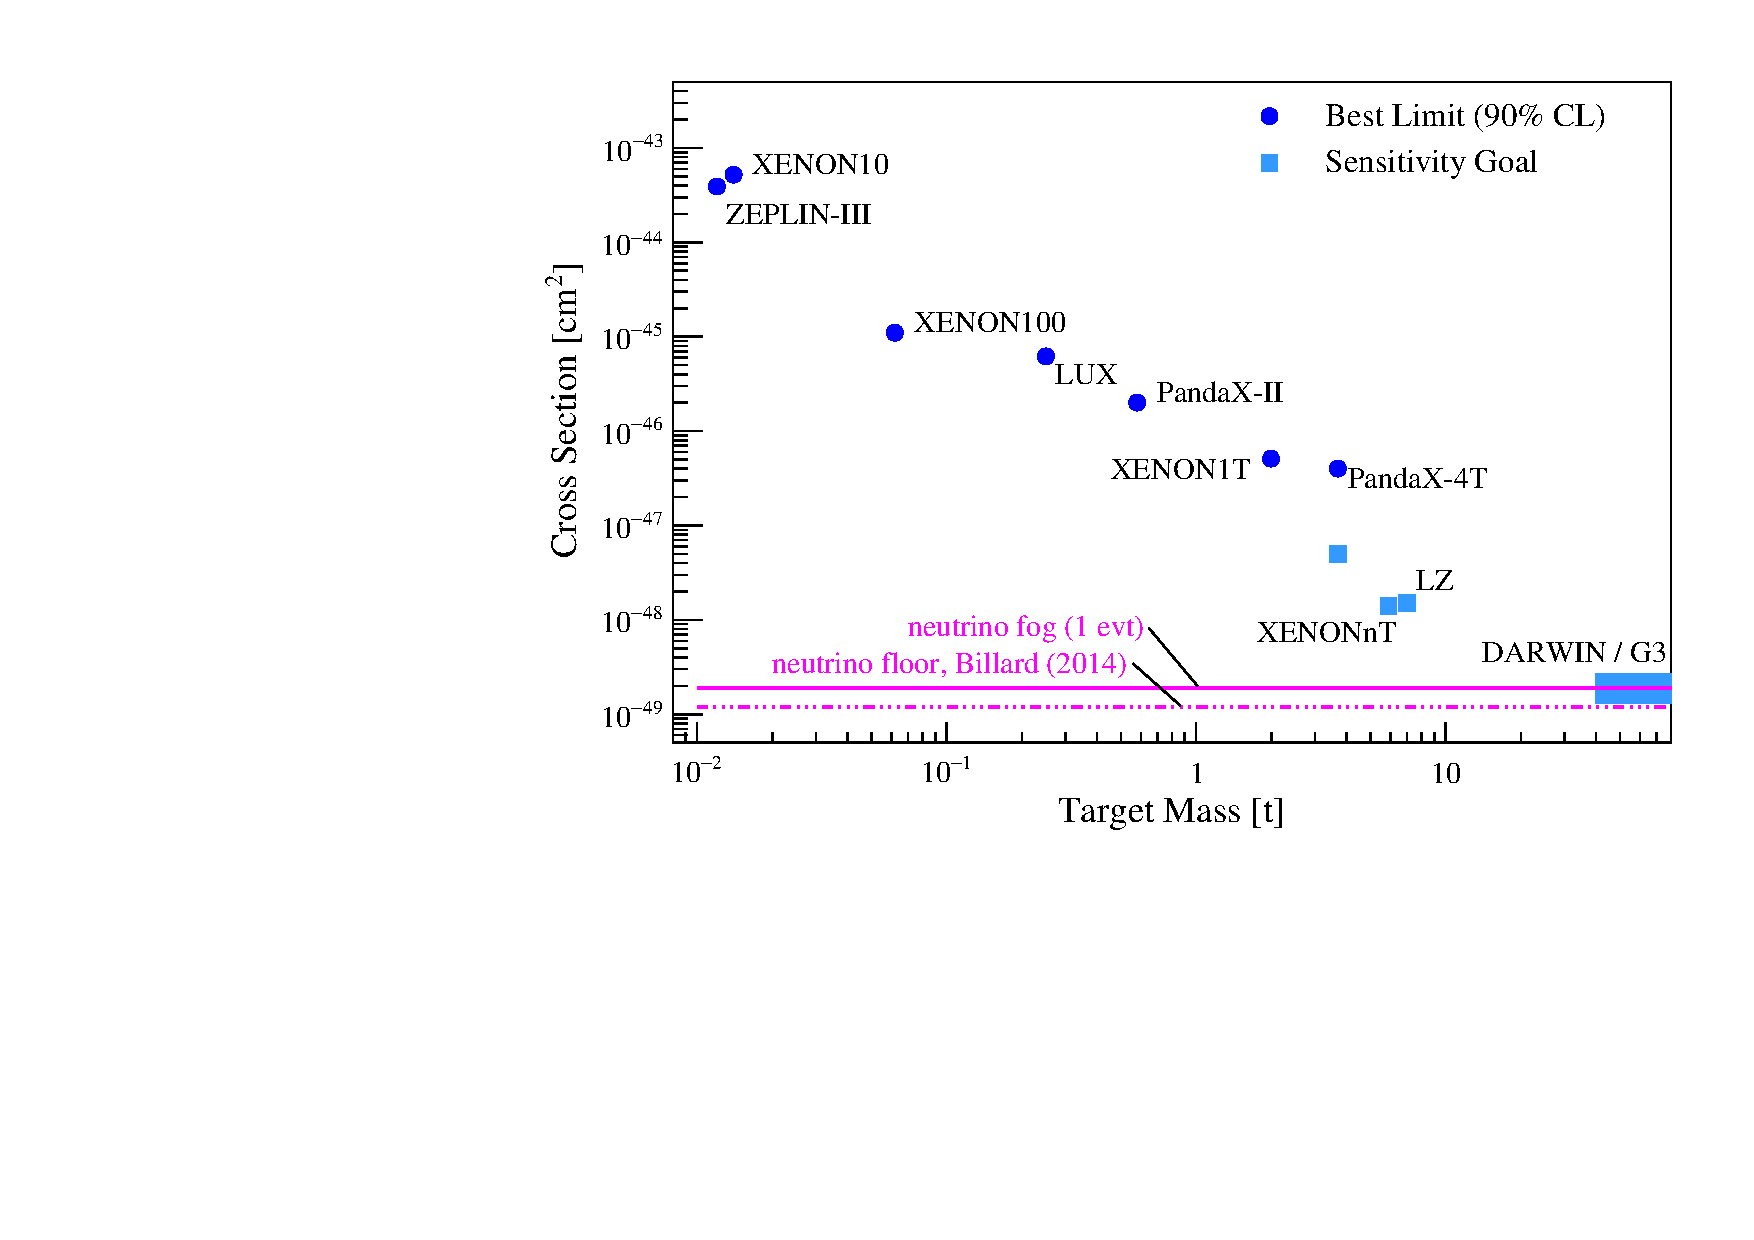
\includegraphics[width=0.48\columnwidth]{figures/xenon_sens_vs_mass.pdf}
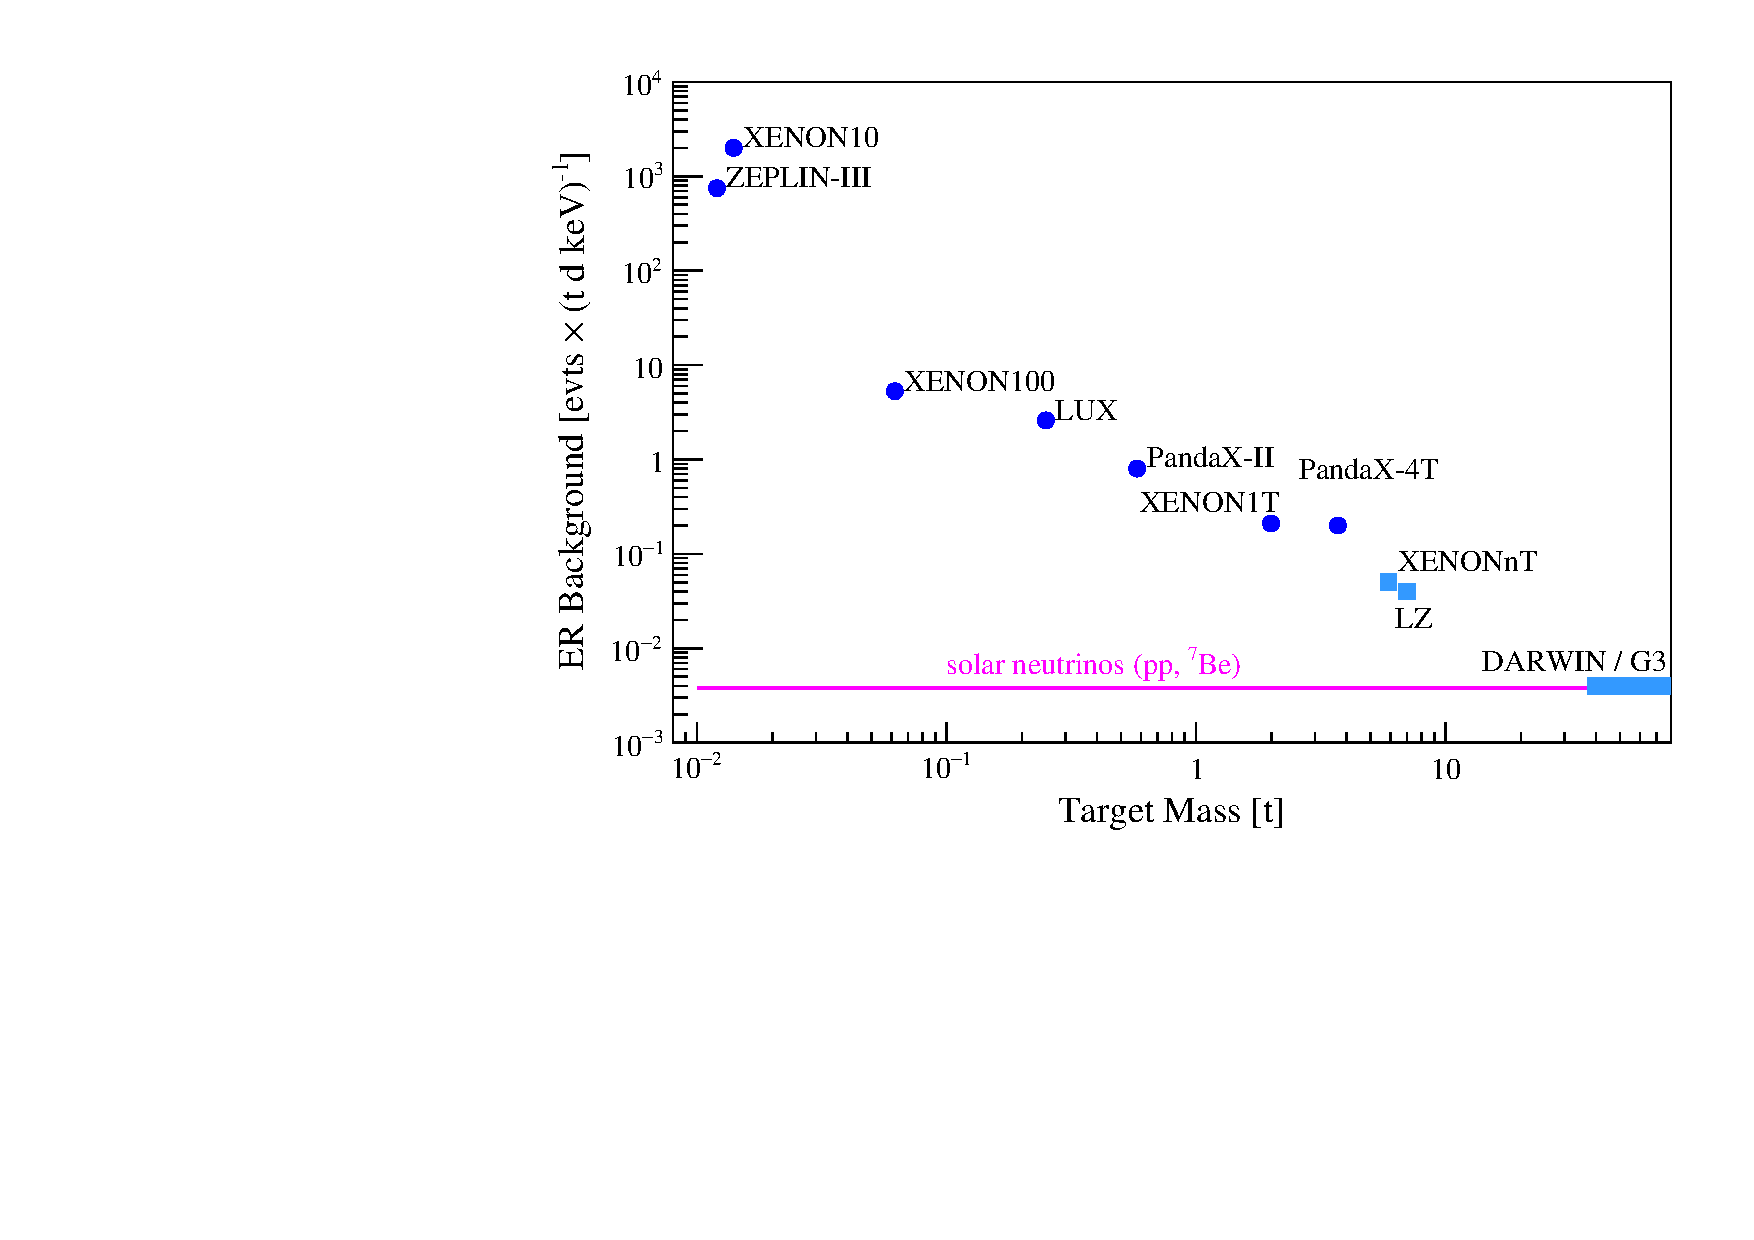
\includegraphics[width=0.48\columnwidth]{figures/xenon_background.pdf}
\caption{Development of the LXe-TPC technology since its inception. The improvement in sensitivity to spin independent WIMP-nucleon coupling achieved by LXe experiments of increasing target masses is shown on the left. The cross section values refers to a WIMP mass of 50~Gev/c$^2$. Sensitivity goals are also reported for experiments that have not yet been completed. The right plot shows, as function of the target mass, the solid progress made in terms of background suppression. The maturity of the technology allowed, at each scale, the identification and characterization of the dominant background sources in the WIMP energy region of interest and the development of techniques capable of efficiently suppressing them for the next phase. Cross section values and background rates are extracted from Ref.~\cite{PhysRevLett.100.021303,PhysRevD.94.122001,AKIMOV201214,PhysRevLett.116.161301,Wang_2020,XENON:2018voc,PandaX:2018wtu,PandaX-4T:2021bab,AKERIB201804,XENON:2020kmp}.
}
\label{fig:xenon_evolution}
\end{center}
\end{figure}

\begin{figure}[!htbp]
\begin{center}
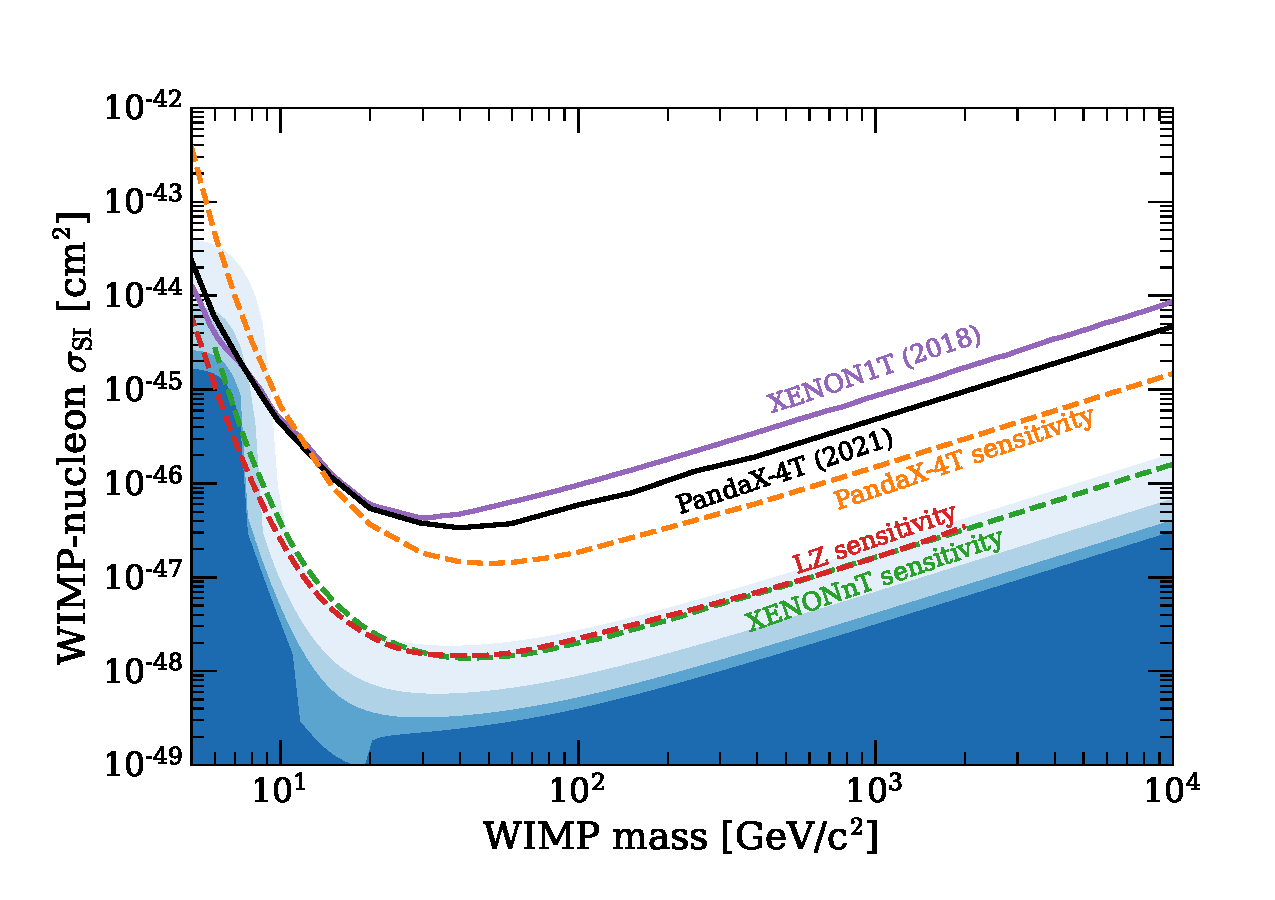
\includegraphics[width=0.99\columnwidth]{figures/xenon_CF1WP1_G2sens_v3.pdf}
\caption{{\color{red}Figure still in progress.} PandaX-4T~\cite{PandaX:2018wtu}, LZ~\cite{AKERIB201804} and XENONnT~\cite{XENON:2020kmp} projected sensitivity to spin-independent WIMP coupling with nucleon compared to XENON1T and PandaX-4T results~\cite{XENON:2018voc,PandaX-4T:2021bab}. The LZ curve is calculated for a 15\,tonne$\cdot$year and with a one-sided upper limit construction. The XENONnT curve is calculated for a 20\,tonne$\cdot$year exposure and with a two-sided interval construction, which is intrinsically less sensitive than the one-sided construction (A 2021 paper authored by members of several dark matter collaborations provided recommendations to ensure that future results are calculated on the same statistical basis~\cite{recommendation_dark_matter}). The PandaX-4T sensitivity is estimated for a 5.6 tonne*year exposure, the PandaX-II detection efficiency, and a cut-and-count signal treatment with 40\% nuclear recoil acceptance~\cite{PandaX:2018wtu}. The blue region represents the neutrino fog, where sensitivity becomes systematics-limited. {\color{red}Refine neutrino fog text after Sec.~2 of this whitepaper has been written.}}
\label{fig:xenon_sensi}
\end{center}
\end{figure}

Two new multi-tonne LXe-TPCs, LZ and XENONnT, are operative since 2021 with a target sensitivity of about 1-2$\times$10$^{-48}$ cm$^2$ (see Fig.~\ref{fig:xenon_sensi}).
The US-European-Japanese collaboration XENON is running the XENONnT experiment at the Laboratori Nazionali del Gran Sasso (Italy). The detector features a 5.9\,tonne LXe target (4.0\,tonne expected fiducial) surrounded by a Gd-doped water Cherenkov active veto to suppress and tag neutron-induced background.

The XENONnT collaboration plans to accumulate a 20\,tonne$\cdot$year exposure. The projected neutrino-induced background rate in the WIMP ROI is of 0.27 events/tonne$\cdot$year and 0.08 events/tonne$\cdot$year for solar and atmospheric neutrino respectively, with the former not affecting WIMP searches for masses larger than 10\,GeV/c$^2$. While the number of events in the WIMP region might be indicative of the background, it does not fully capture the reach of xenon-based detectors where, thanks to the maturity of the technology, the backgrounds are extremely well characterized and modeled in multiple parameter spaces, allowing for a powerful statistical inference process~\cite{XENON:2020kmp}. 
The US-European LUX-ZEPLIN (LZ) experiment is presently operating at Sanford Underground Research Facility (USA) and aims to accumulate a 15\,tonne$\cdot$year exposure~\cite{AKERIB201804}.

The detector features a 7\,tonne target (5.6\,tonne expected fiducial), surrounded by an instrumented LXe skin layer and a Gd-loaded liquid scintillator which together form an efficient anti-coincidence veto and in~situ background monitor. The expected neutrino-induced background rate in the WIMP signal region is 2.35\,events/tonne$\cdot$yr (solar) and 0.02\,events/tonne$\cdot$yr (atmospheric).

About a decade and half of intensive development and deployment has made the LXe-TPC an extremely mature technology capable of being extended to a larger scale with reliable sensitivity projections and consistently solid progress (see Fig.~\ref{fig:xenon_evolution}). Extension of this technology to an even larger scale, enabling systematics-limited exposures, is within reach. A definitive next-generation experiment targeting exposures on the order of 1\,ktonne$\cdot$year would fully explore the accessible WIMP parameter space. The strategy towards such an experiment will be informed by outcomes from the current projects, complemented by a limited and well-defined set of R\&D activities that should take place concurrently. The needed technological improvements appear modest given the limited scale-up that is required with respect to current experiments, less than a factor of two in linear dimensions. 

In China, PandaX-4T is expected to be gradually upgraded into a multi-ten-ton experiment with a nominal fiducial target of 30~ton, to push the sensitivity to dark matter-nucleus coherent scattering to the “neutrino fog” for dark matter masses above 10~GeV/$c^2$. The PandaX collaboration is actively pursuing R\&D for the next generation experiment in parallel with the operation of PandaX-4T until 2025, after which the upgrade is expected to start.

The DARWIN collaboration~\cite{DARWIN:2016hyl}, a successor to XENON, has already started in Europe an intense R\&D program. Given their current leadership roles and expertise, the US teams in both XENONnT and LZ (about 50\% of the community) are well-positioned to contribute significantly to this next-generation effort; in fact, there would be substantial opportunity cost in delaying the US engagement. In 2021, scientists in the LZ and XENON/DARWIN collaborations formally expressed their intent to join forces towards towards this next-generation xenon-based experiment, pursued by a single, joint scientific collaboration~\cite{mou}. While development of a detailed strategy is underway, one potential path forward would foresee a staged project minimizing technological risk at reduced cost, while increasing scientific productivity with an accelerated timeline. A detector design that can be extended along the drift direction would bring substantial benefit:
\begin{itemize}
    \item Minimized technological risk: It would allow in the early phase the operation of a detector that, although compact in its drift direction, would feature full-size electrodes and photo-detector arrays, enabling their characterization directly at the final scale and condition.
    \item Accelerated time to scientific return: It would allow operation of the compact version of the detector, while the full xenon inventory is being procured. 
    \item Reduced cost: A less aggressive timeline for the xenon procurement would enable a meaningful reduction of the project costs, by minimizing impact on the market price of xenon.
    \item Broad user base: It would allow early characterization of the various sources of background in a low background environment, as well as an early science program, to fully engage the next generation of scientists. 
\end{itemize}

The support for a next generation xenon-based experiment extends beyond the new DARWIN/XENON/LZ and PandaX collaborations, as witnessed by the long list of approximately 600 authors signing a recent community white paper outlining the physics reach of such an experiment~\cite{whitepaper_on_the_arxiv_still_in_february}. The large detector scale and low background, combined with many advantageous properties of xenon properties as target, enable a rich science portfolio that extends well beyond WIMPs, transforming such a detector into a cost-effective, broad, low-background astroparticle physics observatory. 